% status: 100
% chapter: Application

\def\paperstatus{100} % a number from 0-100 indicating your status. 100
                % means completed
\def\paperchapter{Application} % This section is typically a single keyword. from
                   % a small list. Consult with theinstructors about
                   % yours. They typically fill it out once your first
                   % text has been reviewed.
\def\hid{hid-sp18-606} % all hids of the authors of this
                                % paper. The paper must only be in one
                                % authors directory and all other
                                % authors contribute to it in that
                                % directory. That authors hid must be
                                % listed first
\def\volume{9} % the volume of the proceedings in which this paper is to
           % be included

\def\locator{\hid, Volume: \volume, Chapter: \paperchapter, Status: \paperstatus. \newline}


\title{Diagnosis of Coronary Artery Disease Using Big Data Analysis}

\author{Hady Sylla}
\orcid{HID339}
  \affiliation{%
  \institution{Indiana University}
  \streetaddress{711 N.Park Ave}
  \city{Bloomington} 
  \state{Indiana} 
  \postcode{47408}
}
\email{hsylla@iu.edu}



\begin{abstract}
  Coronary artery disease (CAD) is the most prevalent heart disease.
  Worldwide, it is among the primary causes of heart failure and
  mortality~\cite{ali}. Therefore, its early diagnosis is essential.
  Specialists have invented different techniques for diagnosing CAD.
  They conduct most of these methods using the Irvine Dataset
  (University of California), which have limitations of features and
  missing values, thus being unreliable. The present study employs big
  data techniques and the latest dataset, with no missing values, and
  with features such as the Q wave, ST depression, functional class, T
  inversion, and dyspnea. This data has been compiled from the Shaheed
  Rajaei Cardiovascular, Medical and Research Center, between 2011 and
  2012, and involves 303 patients. This study uses Naïve Bayes, SMO,
  and a proposed ensemble algorithm, using these features to conduct
  the analyses. Tenfold cross-validation on the dataset has been used
  to design accurate algorithms with an ensemble algorithm, achieving
  88.5\% accuracy. This study extracts the relevant features and rules
  regarding CAD, which previous studies have not discussed.

\end{abstract}

\keywords{\locator\ Coronary disease, big data, Random Forest}

\maketitle

\section{Introduction}

Coronary artery disease (CAD) comes about when atherosclerotic plaques
develop in the coronary arteries, giving rise to a narrowing of the
coronary luminal, and sometimes occlusion, which leads to heart
failure or sudden cardiac failure.In Western nations, CAD is among the
killer diseases.It is essential for people to understand the
pathophysiology of CAD, how to control its development, to identify
any effective innovation in the cardiovascular risk elements, how to
diagnose and treat it in its early stages, and its reversible stages.
Experts have considered big data mining technique as the `gold
standard' for diagnosing CAD, and it is commonly used. However, big
data mining is an expensive and invasive procedure that 
requires a high level of technological expertise and the latest
technology. Thus, medical experts cannot use it to screen or treat
many patients. 
\par For this reason, many health facilities use other noninvasive
tools to diagnose CAD.The most popular of these methods are stress
echocardiography (ECHO), electrocardiogram (ECG), and scintigraphy or
SPECT. Additionally, clinical setups currently use coronary magnetic
resonance angiography (CMRA) MSCT or EBCT. The objective of this study
is to show how to use big data mining technique to diagnose Coronary
Artery Disease and why this is the best way to control heart attacks
and deaths. The review discusses the features in the big data mining
tool, how they derive the results, and presents a discussion of the
results.

Additionally, this paper provides resources for future studies and
offers recommendations to improve the examination of CAD. 
\par Data mining is a technique for finding hidden information in a
database. Nowadays, several fields use data mining; it has different
applications, such as scientific discoveries, entrepreneurship, and
fraud detection. Data mining calculations work on databases in which
each information archive has several attributes. One of these
attributes is the class label, which indicates the  category of the data.  
The data mining algorithms people use in problem solving are
association rule mining, classification, regression analysis,  and
clustering. 
For classification algorithms, there is required a learning phase on a
labeled data set, which requires the researcher to  determine the
missing test record class label. 
In the learning phase, a scientist constructs a classification model
to predict the data label class label using the values  of its features.
A specialist categorizes heart disease into cardiovascular and
cardiomyopathy disorders. 
Coronary Artery Disease (CAD) is a significant cardiomyopathy disease
subgroup, which causes disability, serious illness, and even death, as
the disease affects the supply of oxygen and blood to the heart
muscles. 
\par The early symptoms of heart disease comprise pain in the centre
of the chest or a sense of numbness, and palpitation. Other signs are
fainting fits or dizzy spells, and dyspnea on exertion. Due to the
important nature of heart failures, it is essential to find out its
causes. Currently, the primary goal of many scientific pursuits is
making an accurate diagnosis of cardiac disease. Researchers have
collected a great deal of information while examining CAD patients,
and by processing the data, they can find out how the main features of
cardiac disorders are related (e.g., the amount of cholesterol, blood
pressure, etc.) and the probability of the occurrence of such a
disease. The next chapter discusses several research articles that
discuss this topic and relate it to the findings of the present study.


\section{Contribution of Big Data to Coronary Artery Disease}

This section provides selected examples of the potential of big data
arising from the variety, volume and value of the data people have
obtained. 
Additionally, it shows how big data contribute to scientific advances  
in cardiovascular medicine from the discovery of  underlying disease
mechanisms, disease taxonomy, of treatment relevant  sub-types of the
disease which underpin drug development, and precision  medicine.

\subsection{Discovery in genetic and big data}
Lee, Noh and Ryu~\cite{lee2011ire1} point out that it is challenging
to provide deep mechanistic insight into large-scale big data mining
resources given the limited availability of genetic information in
sufficient depth. 
Bespoke, recallable investigator-led studies, such as East London
Genes \& Health (ELGH) and the NIHR BioResource enable the  coupling
of big data mining with extreme genotypes and facilitate  their
in-depth study using bespoke experimental protocols. 
Complete gene knockouts inform people about the gene process. 
With the latest survey of 3,222 British Pakistani-heritage exome
sequenced persons with high parental relatedness, there have  been
discovered 1,111 rare-variant homozygous most likely  function loss
(rhLOF) genotypes to predict the disruption (knockout) of  781 genes
\cite{wang2005framingham}. 
\par Rajkumar~\cite{rajkumar2010diagnosis} stated that linking big
data to the rhLOF genotypes is not associated with a doctor or
prescription consultation rate, and there are no illness-related
phenotypes in 33 out of 42 individuals with rhLOF genotypes in
Mendelian recessive complexity genes. Phasing the genome sequencing of
a healthy PRDM9 knockout woman, her controls, and baby, found meiotic
recombination sites localized from the hotspots with PRDM9 dependency,
depicting PRDM9 redundancy in human beings. There have been genomic
approaches to validating case definitions: across thousands of
hospital ICD codes, there have been reproduced associations from
genome-wide association studies obtained one phenotype at a time.

\subsection{Discovery in larger scale epidemiology}
Big health records data can contribute to the discovery of new
associations which would be hard to generate from traditional
consented cohorts without record linkage. 
 This involves a resolution across a range of risk factor levels and a
 range of different initial presentations of cardiovascular disease.
 Various associations have been discovered in a cohort of more than
 one million adults initially free from diagnosed cardiovascular
 disease using national structured linked electronic health records
 from the CALIBER resource, in which EHR phenotyping algorithms are
 created, validated and shared using a robust methodology
~\cite{wang2005framingham}. Sideman~\cite{sideman1985simulation}
 argued that the primary necessity for precision medicine is
 estimating the patient's state. The experts mainly analyze the
 correlations of illness trajectories with a focus on a few
 complications or by the use of large-scale techniques without taking
 time into consideration. Researchers have performed a
 discovery-driven study of illness progression patterns using data
 from an electronic health registry covering the entire population of
 Denmark. Using the whole illness spectrum, they created 14.9 years of
 records data for 6,200,000 patients for 1,171 critical trajectories.
 Those experts identified primary diagnoses, such as chronic
 obstructive pulmonary disease and gout obstructive pulmonary disease,
 as the cause of the progression of CAD across many of these paths.
 Thus, it is of added significance to diagnose CAD earlier. Such a
 data-driven approach analysis is useful for preventing and predicting
 future complications in individual patients
~\cite{sideman1985simulation}.

\subsection{Discovery with deep phenotypic data}

Most cardiovascular diseases (including acute myocardial infarction)
have syndromic descriptions and labels, which may span multiple
underlying pathological disease processes. One approach to discovering
the mechanistically relevant disease types is to phenomenal the
disease~\cite{sahaf2011comparing}. For example, in heart failure with
preserved ejection fraction, machine learning in 46 continuous
clinical, laboratory, electrocardiographic, and echocardiographic
findings have determined mutually exclusive groups related to the
subsequent outcomes. The cardiac atlas project (of healthy and
diseased hearts) is an example of a large-scale collaboration on
feature extraction in imaging, using data sharing in standard formats
Digital Imaging and Communications in Medicine (DICOM) of the pixel
and non-pixel data. Personalization using physiological simulations,
for example, for cardiac resynchronization therapy, has been proposed.
Unstructured free-text data in big data mining adds a further way to
estimate disease co-occurrence and patient stratification, which
people map to the biological frameworks of systems
\cite{sahaf2011comparing}.


\subsection{Discovering and validating drug targets}

Regarding a discussion by~\cite{rajkumar2010diagnosis}, big data-DNA
resources may play an increasingly important role in drug discovery,
genomic drug target validation, marker validation, and drug
repurposing. For example,~\cite{rajkumar2010diagnosis} demonstrates a
strategy in which human mutations that inactivate a gene encoding a
drug target can mimic the action of an inhibitory drug, here
ezetimibe, and thus can be used to infer potential effects of that
drug. Ezetimibe is known to affect the marker (LDL cholesterol) but,
until recently, not the disease (myocardial infarction). Among the
most significant sources of cases of MI and controls in this study was
a DNA resource integrated into a health system with rich big data. The
discovery of PCSK9 as a drug target to lower cholesterol, which the
EHR-DNA resources make in principle, illustrates the importance of
rare variants in the identification of pathways relevant to the whole
population. Mendelian randomization studies are essential in
evaluating whether markers, such as heart rate and HDL cholesterol,
are causal for the disease of interest. Such genetic studies have
questioned the role of heart rate and HDL cholesterol in the etiology
of heart attack~\cite{Wijeysunderae000731}.

\subsection{Cost effectiveness of innovation}

The Institute of Medicine (U.S.), Institute of Medicine (U.S.), and
Institute of Medicine (U.S.) (2011) shows that big data provide new
opportunities for understanding the cost-effectiveness of existing and
new interventions. Because of the ability to assess baseline risks in
unselected general populations (usually a higher risk than those
reported in trials), such `real world evidence' is increasingly
required by payers and regulators. As more data sources are linked,
greater granularity of the care data (e.g., 67 different types of
primary care `consultation') may provide more accurate and more
complete resource use data. For example, cost-effectiveness decision
models can be developed before trials, reporting an estimate of the
willingness to pay and pricing of a drug according to different trial
benefits (relative risk reductions) applied to patients at various
strata of risk~\cite{breiman2001random}.

\subsection{Public health}

Agrawal~\cite{agrawal1993mining} assert that there are significant
gaps in our ability to prevent the onset of and prolong life in, many
of the most common cardiovascular diseases in the 21st century
including atrial fibrillation, heart failure, and peripheral arterial
disease. There are also gaps in our ability to measure disease and
model the impact of interventions in populations. Clinicians diagnose
more specific entities than `heart attack', `CHD' or `CVD,' yet
conventional consented cohorts have lacked the statistical size or the
phenotypic resolution to measure clinically relevant sub-types of
disease~\cite{chu2009bayesian}. Big data can study the conditions that
clinicians diagnose to provide scalable, population-based, updatable
measurements of new disease burden vital for the evaluation of
alternative strategies of prevention. For example, significant data
can be used to estimate the incidence and survival of the
treatment-relevant sub-types of MI (ST elevation and non-ST elevation)
\cite{dietterich2000ensemble}.

\section{Analysis}

To characterize the algorithms, a researcher requires a learning stage
on a labeled dataset collection, which makes it possible to settle on
the missing test record class~\cite{ali}. 
In the learning stage, a researcher builds an order model to predict
the data label class label using the values of its features. 
A specialist categorizes heart diseases as cardiovascular and
cardiomyopathy disorders~\cite{ali}. 
Coronary Artery Disease (CAD) is a noteworthy cardiomyopathy
inconvenience subgroup which causes inability, genuine sickness, and
even death, as the disease affects the supply of  oxygen and blood to
the heart muscles. 
The early indications of coronary illness involve torment in the focal
point of the chest or a feeling of deadness, and palpitation. 
Different signs include blacking out fits or spells of feeling mixed
up, and dyspnea on the effort. 
\par Due to the vital importance of heart failure, the primary goal of
many scientific pursuits is to make an accurate diagnosis of cardiac
diseases. Analysts have gathered a lot of data while looking at CAD
patients, and by preparing the information, they have uncovered how
the main features highlighting cardiovascular issues are related
(e.g., the measure of cholesterol, circulatory strain, and so on) and
the probabilities of the occurrence of these diseases.

\subsection{Dataset}

<A dataset constructed from the information collected from 303 random
visitors (216 patients) to the Shaheed Rajaei Cardiovascular, Medical
and Research Center was used to evaluate the effects of different
demographic, clinical, and ECG features on the diagnosis of coronary
artery disease. This dataset is publicly available and does not
contain any patient identifiers. Demographics, such as age and sex,
are also included in the dataset.

\subsection{Method}

I will use Random Forest machine learning for predicting the features
to diagnose coronary artery disease. Random Forests (RF) is a
prominent tree-based ensemble machine learning tool that is
exceptionally data adaptive~\cite{breiman2001random}. I will primarily
be using the SciPy stack, especially pandas, matplotlib, seaborn, and
sklearn. I use the \verb|describe()| method, which gives me the basic
statistics for every column in the dataset. This method will allow me
to generate descriptive statistics that summarize the central
tendency, dispersion, and shape of a dataset.

\begin{table}
\centering
\caption{Dastaset Description}
\label{my-label}
\begin{tabular}{llllllllllllllllllllll}
Age & Weight & Length & Sex & BMI   & DM        & HTN & Current Smoker & Ex-Smoker & FH & ...
& K   & Na  & WBC & Lymph & Neut & PLT & EF-TTE & Region RWMA & VHD & Cath   &        \\
0   & 53     & 90     & 175 & Male  & 29.387755 & 0   & 1              & 1         & 0  & 0   & ...
& 4.7 & 141 & 5700  & 39   & 52  & 261    & 50          & 0   & N      & Cad    \\
1   & 67     & 70     & 157 & Female & 28.398718 & 0   & 1              & 0         & 0  & 0   & ...
& 4.7 & 156 & 7700  & 38   & 55  & 165    & 40          & 4   & N      & Cad    \\
2   & 54     & 54     & 164 & Male  & 20.077335 & 0   & 0              & 1         & 0  & 0   & ...
& 4.7 & 139 & 7400  & 38   & 60  & 230    & 40          & 2   & mild   & Cad    \\
3   & 66     & 67     & 158 & Female & 26.838648 & 0   & 1              & 0         & 0  & 0   & ...
& 4.4 & 142 & 13000 & 18   & 72  & 742    & 55          & 0   & Severe & Normal \\
4   & 50     & 87     & 153 & Female & 37.165193 & 0   & 1              & 0         & 0  & 0   & ...
& 4.0 & 140 & 9200  & 55   & 39  & 274    & 50          & 0   & Severe & Normal
\end{tabular}
\end{table}


For a better visualization of the data, I will generate a histogram.
Data visualization facilitates the interpretation and breaks down big
data in a manner that is easily understandable. 

\begin{figure}
    \centering
    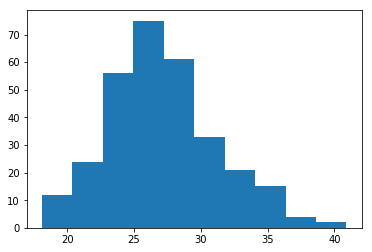
\includegraphics[width=1.0\columnwidth]{images/output_2_0.png}
    \caption{Bar Plot}\label{Plot}
\end{figure}



\subsection{Data Preparation}

Since this dataset includes string data, I will use encoding to
transform the categorical features to a format that works better with
classification by taking all categorical features that have only two
levels and label-encode them to get binary features.

\begin{figure}
    \centering
    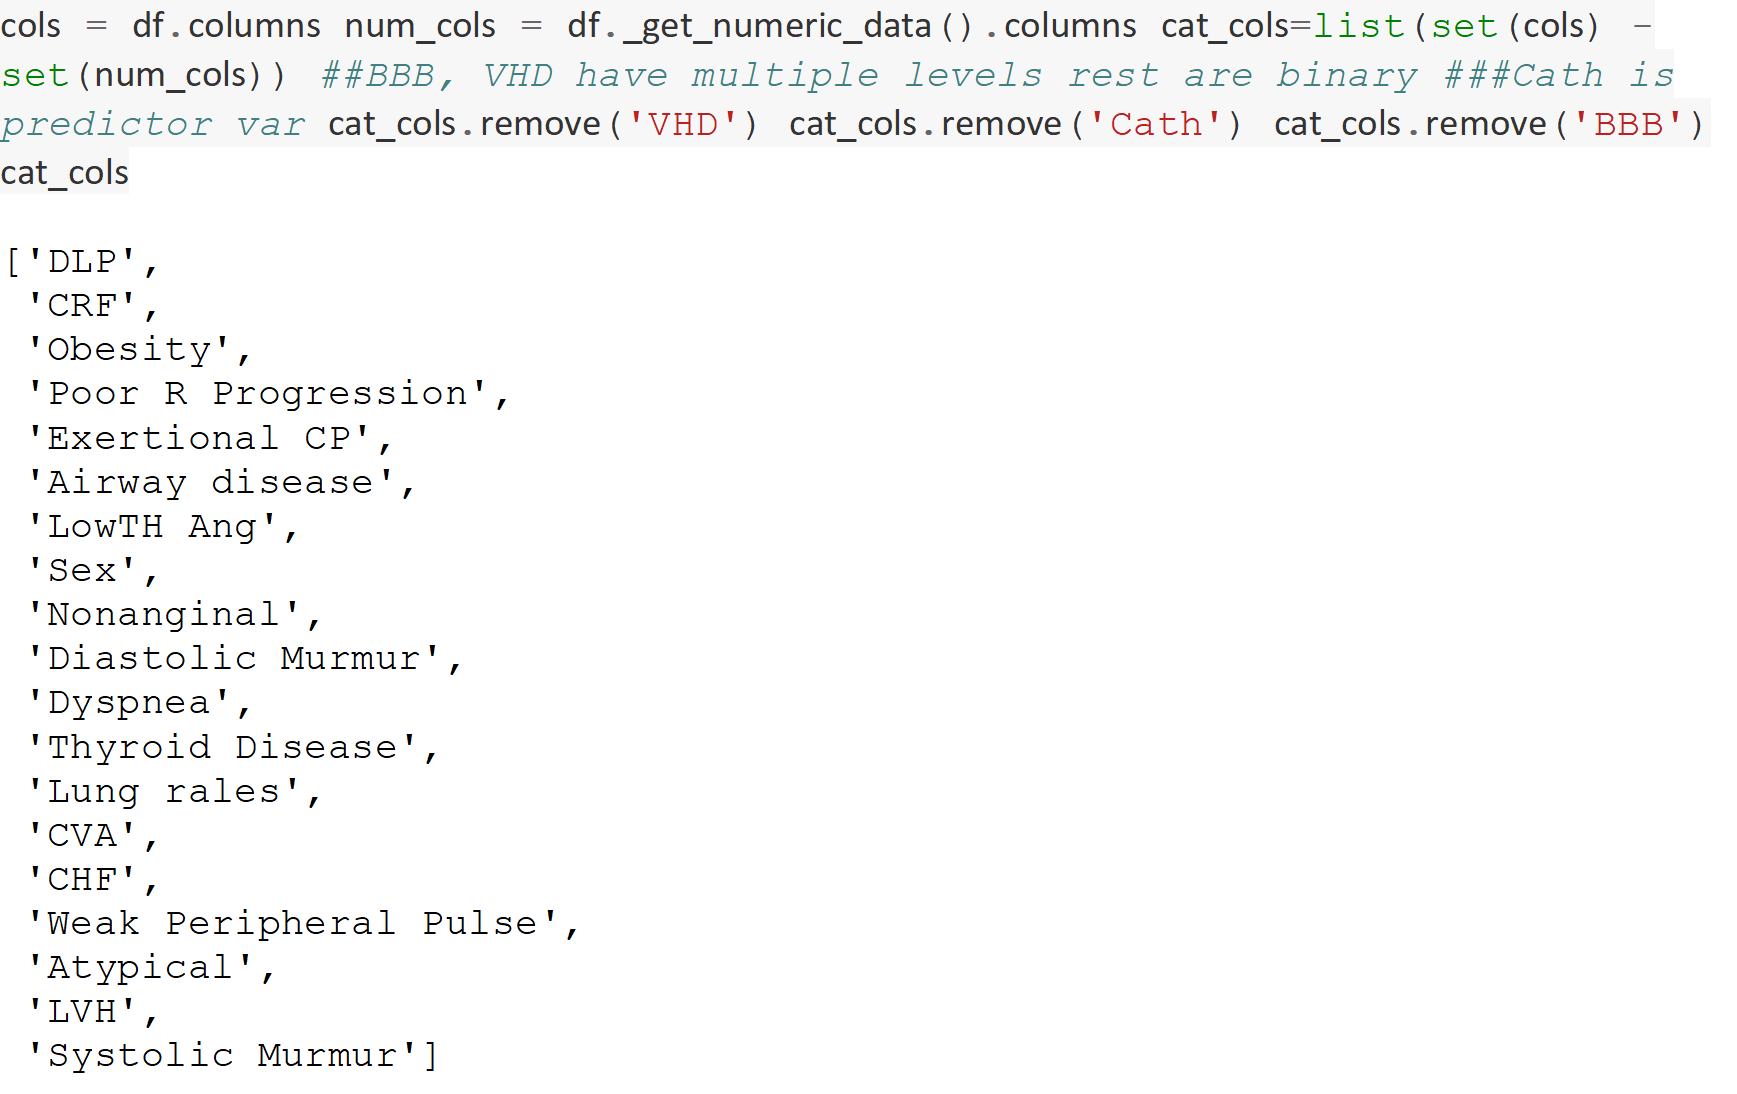
\includegraphics[width=1.0\columnwidth]{images/Untitled3.png}
    \caption{Encoding}\label{Encoding}
\end{figure}

Then I will apply one hot encoding to our multiple level features,
that will allow the representation of categorical data to be more
expressive.

\begin{figure}
    \centering
    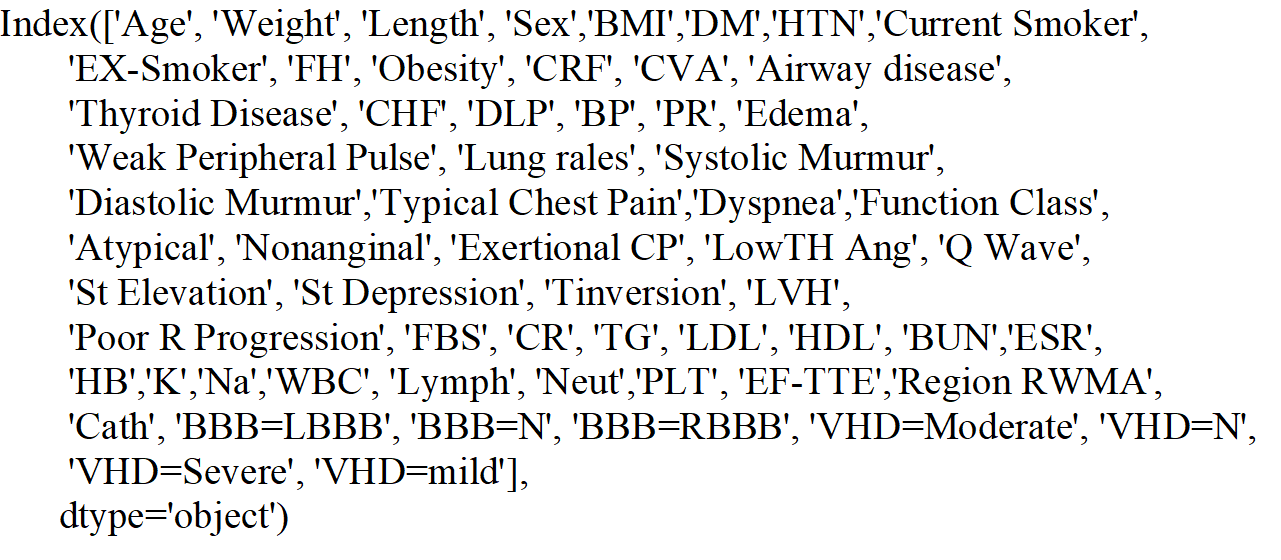
\includegraphics[width=1.0\columnwidth]{images/Encoding.png}
    \caption{Hot Encoding}\label{Hot Enco}
\end{figure}
    
\subsection{Measure of Variable Importance Ranking}

An essential element of RF is that it gives a quickly calculable inner
measure of the significance of a variable (VIMP) that can be used to
rank the factors. This is particularly valuable for high-dimensional
genomic information. In spite of the fact that there are numerous
fruitful applications using change significance, a drawback is that it
is a ranking-based approach. Ranking is significantly more troublesome
than the variable determination issue, which just tries to choose a
group of factors that when consolidated are prescient, without forcing
a positional structure. In any case, in view of the many-sided quality
in organic frameworks, positional quality records in light of RF or
RSF which consider relationship and communication impacts are still an
immense change from univariate positioned quality records in light of
the $t$-test's or Cox corresponding peril occurring when utilizing one
variable at any given moment. Be that as it may, caution is required
when deciphering any straight positioning since it is as a rule likely
that various arrangements of feebly prescient highlights are mutually
prescient. This seems, by all accounts, to be an uncertain issue of
positioning, and further investigation is required. I will specify
which dataset and variable I want to predict. I like to keep a
parameter file where I specify data sources and such. This lets me
create generic analytics code that is easy to reuse. After I have
specified what dataset I want to study, I split the training and test
datasets. Then I will scale the data, which makes most classifiers run
better.

\begin{figure}
    \centering
    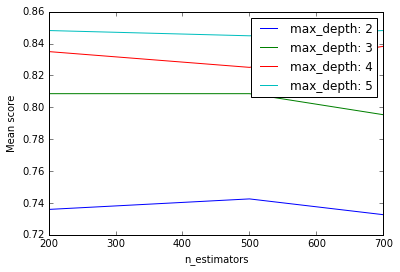
\includegraphics[width=1.0\columnwidth]{images/output_15_1.png}
    \caption{Scores Attribute}\label{Score}
\end{figure}

\begin{figure}
    \centering
    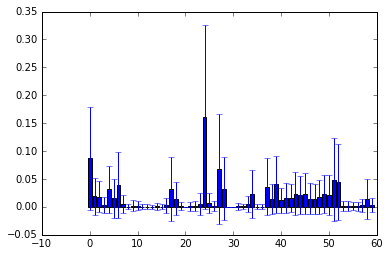
\includegraphics[width=1.0\columnwidth]{images/output_17_0.png}
    \caption{Feature importance with their standard deviations}\label{Featites Format}
\end{figure}

\begin{table}
\centering
\caption{Feature Importance Table}\label{Importance}
\begin{tabular}{lll}
Importance            & Std      &          \\
Age                   & 0.086779 & 0.092552 \\
Weight                & 0.018672 & 0.032956 \\
Length                & 0.018183 & 0.027928 \\
Sex                   & 0.003414 & 0.013603 \\
BMI                   & 0.031609 & 0.042215 \\
DM                    & 0.015427 & 0.034442 \\
HTN                   & 0.038735 & 0.059296 \\
Current Smoker        & 0.005287 & 0.015965 \\
Ex-Smoker             & 0.000587 & 0.004463 \\
FH                    & 0.002472 & 0.010216 \\
Obesity               & 0.002333 & 0.008439 \\
CRF                   & 0.000534 & 0.004805 \\
CVA                   & 0.000469 & 0.004108 \\
Airway disease        & 0.000474 & 0.003385 \\
Thyroid Disease       & 0.001086 & 0.006045 \\
DLP                   & 0.000407 & 0.004046 \\
BP                    & 0.003296 & 0.013382 \\
PR                    & 0.031988 & 0.056958 \\
Edema                 & 0.014277 & 0.029568 \\
Weak Peripheral Pulse & 0.001758 & 0.007496 \\
Lung rales            & 0        & 0        \\
Systolic Murmur       & 0.001332 & 0.007931 \\
Diastolic Murmur      & 0.001853 & 0.008916 \\
Typical Chest Pain    & 0.00495  & 0.020264 \\
Dyspnea               & 0.161378 & 0.165277 \\
Function Class        & 0.006237 & 0.01781  \\
Atypical              & 0.001798 & 0.008412 \\
Nonanginal            & 0.067681 & 0.098911 \\
Exertional CP         & 0.032299 & 0.056285 \\
LowTH Ang             & 0        & 0        \\
Q Wave                & 0        & 0        \\
St Elevation          & 0.000976 & 0.005923 \\
St Depression         & 0.005336 & 0.014798
\end{tabular}
\end{table}

By checking the model's accuracy on the test set, as shown in the
figure below, the accuracy score on the test by Random Forest attained
0.8852.

\begin{figure}
    \centering
    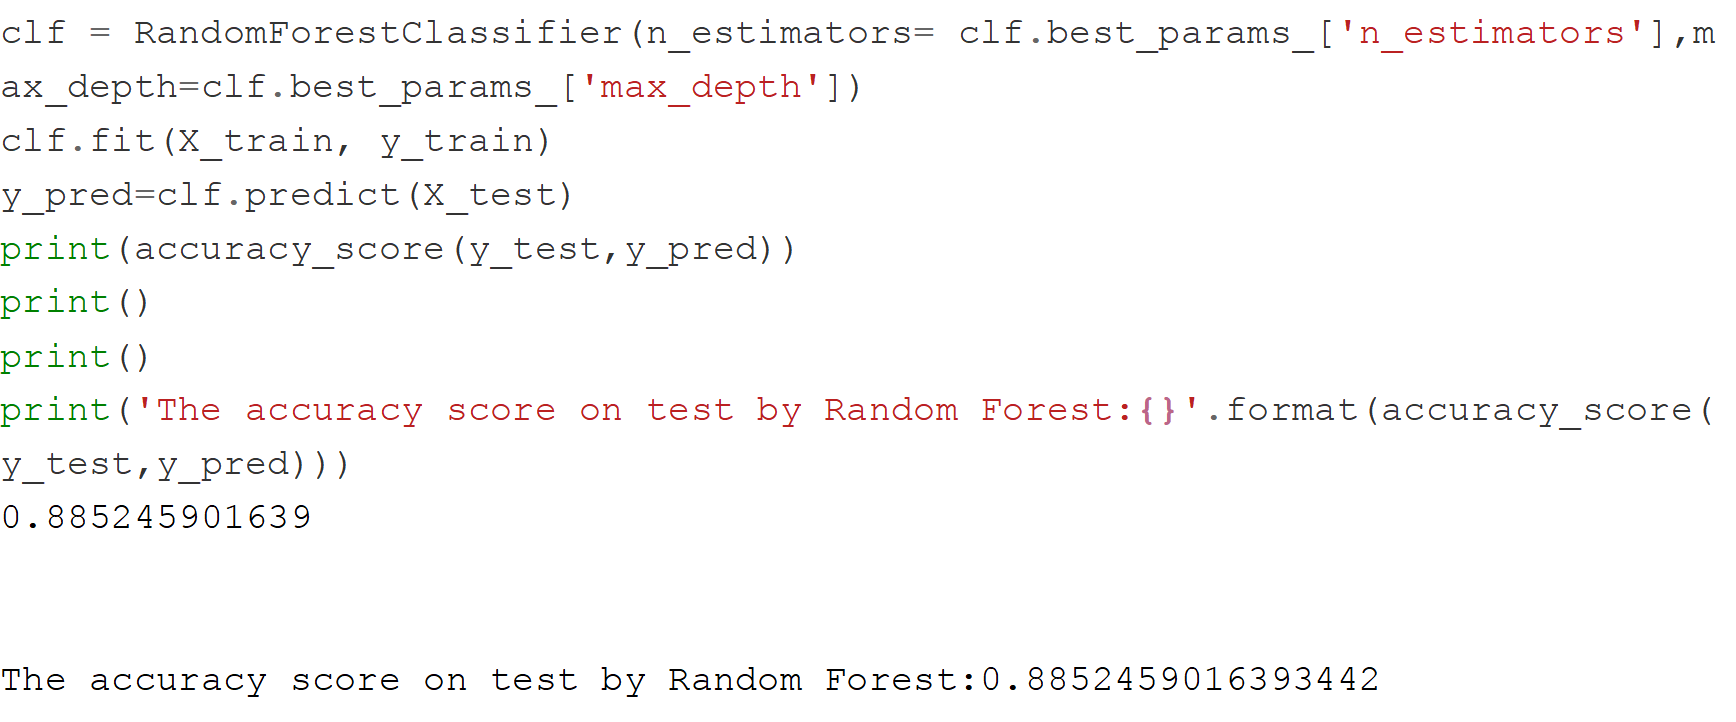
\includegraphics[width=1.0\columnwidth]{images/Untitled7.png}
    \caption{Accuracy Test}\label{Accuracy}
\end{figure}



\section{Conclusion}
This research uses a new dataset, comprising 38 features, together
with data mining methods, to get useful results about this  area of
research. Afterward, the study chooses 16 features using an element 
selection algorithm and some common classification algorithms, and
applies the proposed ensemble algorithm to the dataset. 
The research obtains the highest accuracy (88.51\%) when both the
element selection algorithm and the ensemble algorithm are  used.
Additionally, the study uses association rule mining methods to
extract rules of high confidence from the dataset. 
Coronary Artery Disease (CAD) is among the primary causes of death in
the world. 
Thus people must put measures in place to predict, treat, and control
this disease. 
The use of big data mining techniques will help achieve this and,
therefore, reduce the  mortality rate of people with this disease.
Additionally, not only should medical experts know the use of this
technique, but the  entire community, because heart failures happen at
unexpected times. 
\par The objectives of future studies should include adding other
features, such as echo and lab echo data, to investigate the effect of
these elements on CAD diagnosis and get a higher accuracy in
predicting the progression of this disease. Furthermore, future works
should use more algorithms and data mining techniques to improve the
findings. Lastly, studies should extend the dataset with more sick
people who can help in finding interesting results which may not be
apparent for the patients in the dataset used here. Another aim of
future research should be simplifying the use of big data mining
methods to make them user friendly; this will make many medical
facilities adopt the idea. Moreover, future studies should research
other tools that can improve the big data mining technique's process,
thus making it less costly and require less technological know-how.

\section{Recommendations for Future Studies}

Many nations in the world have big data mining systems that research
can use.  Hence, to enable the research potential of these information
sources, these countries have to centralize the resources that govern
the research dataset. 
Some states have initiatives towards achieving this, although few
tackle all the elements of this procedure. 
For example, the CALIBER platform, which is in the United Kingdom,
joins a repository of big data mining phenotypes with curated
registered linkages combining disease registry (Myocardial Ischaemia
Nation Audit Project). 
Additionally, it joins primary care (Clinical Practice Research
Datalink), death registry (Office of National Statistics), and
hospital discharge (Hospital Episode Statistics) data for over two
million adults with ten million individuals’ follow-up years. 
However, this resource does not offer tools for bidirectional
relations with big data mining information sources. 
The United States National Human Genome Research Institute-funded
consortium, the eMERGE Network, combines big data mining with a
phenotype repository from multiple secondary healthcare systems,
including text and imaging, joined to genotypic data for all
candidates. 
Lastly, the Clinical Record Interactive Search system, which is at the
Maudsley NHS Foundation Trust, NIHR Mental Health Biomedical Research
Center and Dementia, and South London's Dementia Unit also help
researchers. 
The Clinical Record Interactive Search system allows scholars to
analyze secondary data, comprising clinical notes and other texts,
through simple tools that help to identify patients meet specific
criteria, and help develop text-mining algorithms. 
\par Regarding this, the national big data mining portals can join the
strengths of these projects by including: (i) Standards-driven types
of equipment that enable reviewers to create interventional and
observational studies; 
(ii) A countrywide catalog of contemporary big data mining sources
which is metadata standards curated; 
(iii)  Big data mining phenotype algorithms with an interactive
thesaurus. 
By accomplishing this, the national catalog can support metadata
integration and harvest from manually curated and external sources by
researchers within a reproducible and standardized framework, and also
offer a guide to the data content and access. 
In this way, users will be able to find sources of information that
provide data both across and within disease areas. 
\par The creation of big data mining datasets and algorithms should be
implemented in a way that supports modification and reuse by other
users, as well as the academic citation and credit that is
appropriate. Creating this form of resource enables fostering an `open
source' approach to big data mining research in which researchers
learn and collaborate with one another. It will eventually produce an
advance in big data mining, more than any other research group in
isolation can achieve.


\begin{acks}
The authors would like to thank Professor Gregor von Laszewski and his
team for assistance in providing me the tools and  knowledge to
complete this project. 
\end{acks}

\bibliographystyle{ACM-Reference-Format}
\bibliography{report} 


\newpage
\appendix
\section{Code Reference}
All code and files for this project can be found in the Githup repository:
\url{https://github.com/bigdata-i523/hid339/blob/master/project/code}


